\documentclass[11pt]{article}
\usepackage[margin=1in]{geometry}
\usepackage[T1]{fontenc}
\usepackage[utf8]{inputenc}
\usepackage{lmodern}
\usepackage{microtype}
\usepackage{hyperref}
\usepackage{enumitem}
\usepackage{setspace}
\usepackage{xcolor}
\usepackage{graphicx}

\hypersetup{
  colorlinks=true,
  linkcolor=black,
  urlcolor=blue,
  citecolor=black,
  pdftitle={Speedrunning Social Development: How We Can Improve How We Improve},
  pdfauthor={Tyler Roost}
}

\setlength{\parskip}{0.65em}
\setlength{\parindent}{0pt}
\setlist[itemize]{topsep=0.35em,itemsep=0.25em,leftmargin=1.6em}
\setlist[enumerate]{topsep=0.35em,itemsep=0.25em,leftmargin=1.8em}

\title{Speedrunning Social Development: How We Can Improve How We Improve\\\large v0.2}
\author{Tyler Roost}
\date{}

\begin{document}
\maketitle

\begin{abstract}
Digital platforms shape an increasing share of human social development: how people communicate, learn, coordinate, create, belong, and build identity. Yet most platforms are still optimized through blunt proxies such as engagement, retention, conversion, and monetization. Those metrics can be useful, but they do not reliably tell a platform how to become better at becoming better. They help a system extract value. They do not necessarily help it learn.

This paper presents a \textbf{paradigm-shifting conceptual framework} for the meta-improvement of digital products and digital social infrastructure. The core claim is that platforms should not only optimize user-facing experiences; they should also optimize the mechanisms by which they discover failure, absorb criticism, reward valuable contributors, redesign their own metrics and ranking systems, and personalize user experience through trajectories of use rather than static segmentation alone. The framework combines a user-satisfaction hyper-objective, structured rating-plus-feedback loops, layered contributor incentives, feedback-user training, leaderboard critique, glitch-hunting subcultures, and a four-part hypertopology of learning: \textbf{Human-Compliant, Human-Adversarial, Tool-Compliant, and Tool-Adversarial}.

The comparison point is speedrunning. Long-lived speedrunning communities are resilient because they know how to metabolize breakage. A new exploit does not automatically destroy the scene. It often creates new categories, new routes, new verification norms, and deeper collective understanding. This paper argues that digital platforms should do the same. For builders, this means more robust product learning. For project managers, it means a cleaner loop from user signal to roadmap decisions. For investors, it means a stronger theory of compounding product quality and better investment judgment through lower dependence on internal fiction and proxy blindness, with upside not only for revenue quality but also for cost reduction and profit quality.
\end{abstract}

\section{Introduction}

The digital systems through which people live increasingly function as developmental environments. A social network, chatbot, game, productivity tool, streaming platform, or communication surface is not just software. It is part of the social environment in which people form habits, relationships, identities, skills, expectations, and beliefs about what is possible.

If these environments are optimized badly, millions of people experience shallow, manipulative, or confusing systems as normal. If they are optimized well, the quality of social life can improve at scale.

The usual explanation for digital decay is human nature: people are status-seeking, distractible, tribal, impulsive, and easy to manipulate. This explanation contains some truth but is too incomplete to be useful as a design philosophy. The deeper issue is that most platforms do not actually know how to learn from their own failure modes beyond a narrow set of business proxies. They are optimized to survive, grow, and monetize, but not to become increasingly wise about what their users value, how their incentive systems distort behavior, or how their own internal metrics can be gamed.

This paper proposes a different design frame: a platform should be treated as a system that must learn \textbf{how to improve how it improves}. It is offered as a paradigm-shifting conceptual framework rather than as a conventional empirical paper. Its goal is not to bury the reader in exhaustive measurement before the design space is visible. Its goal is to formalize a stronger design target first, then make empirical testing easier to structure later.

That shift matters at every layer of a company.

For builders, it means product architecture should support not just features, but learning loops.

For project managers, it means the roadmap should be informed not only by raw feedback or analytics, but by increasingly structured, contestable, and high-value feedback. It also reduces \textbf{internal fiction}: internal metrics, narratives, or coordination stories that help the company cohere but do not reliably track user-valued improvement.

For investors, it means product quality can be understood as a compounding capability rather than a static artifact. The strongest products are not just good. They are good at learning why they are not good enough yet, and they can often lower operational waste while doing so.

\begin{figure}[t]
\centering
\IfFileExists{figures/traditional_vs_speedrunning_development_approaches.png}{%
  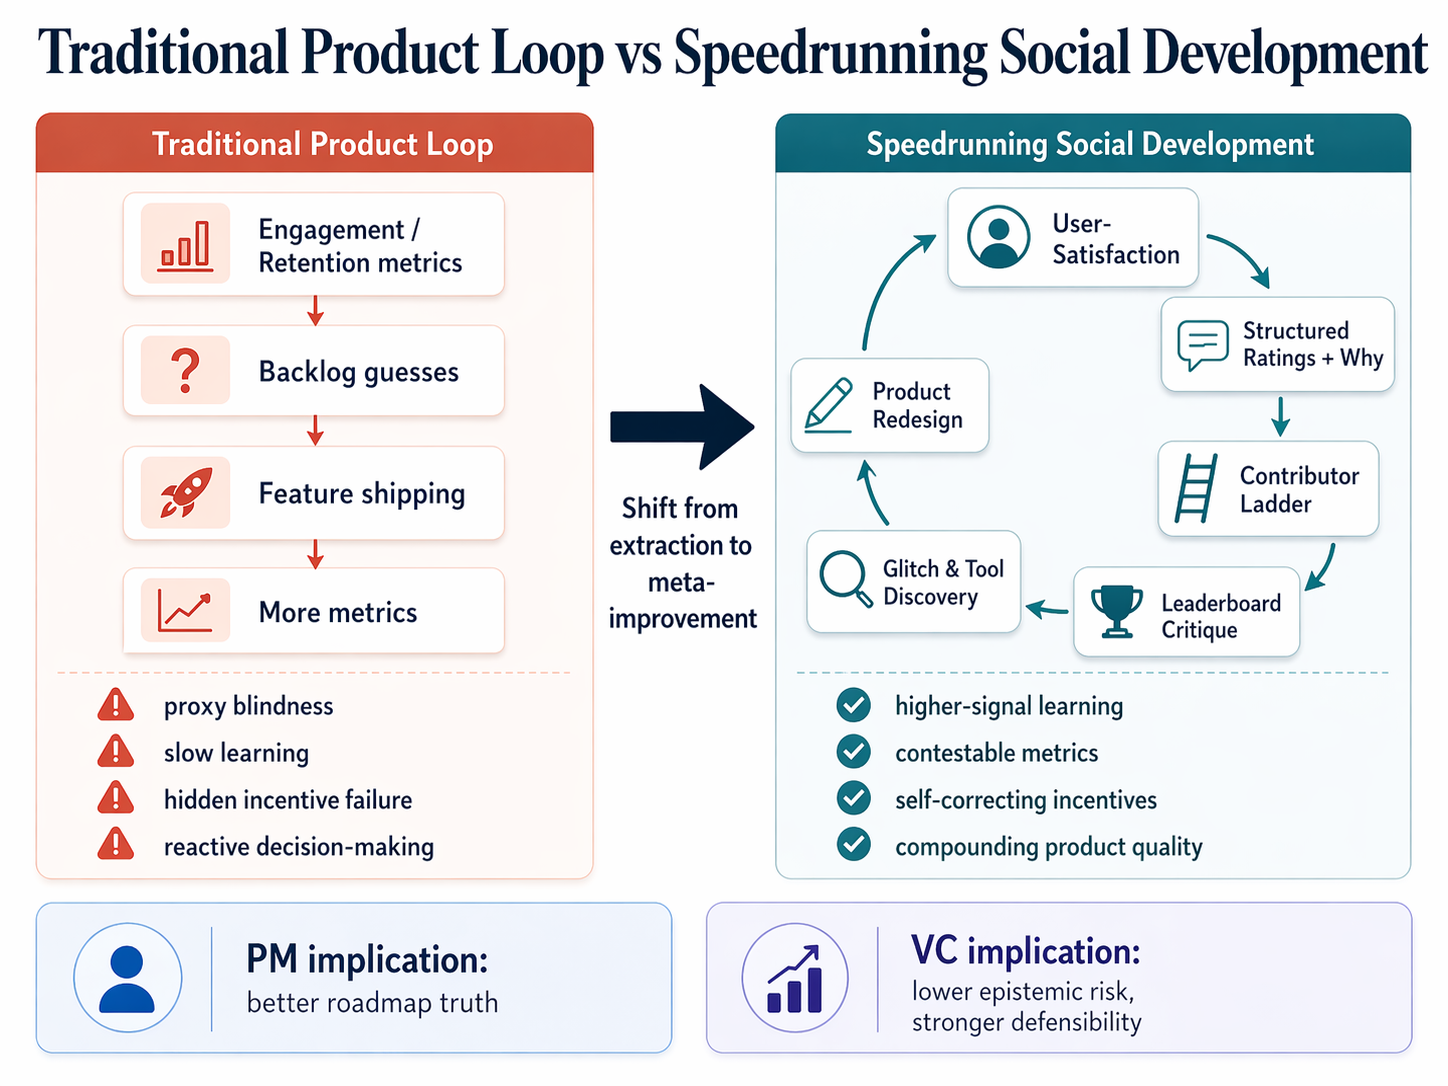
\includegraphics[width=\textwidth]{figures/traditional_vs_speedrunning_development_approaches.png}
}{%
  \fbox{\parbox{0.95\textwidth}{\centering
  Figure placeholder: add \texttt{figures/traditional\_vs\_speedrunning\_development\_approaches.png} to render the selected comparison diagram in the canonical PDF.}}
}
\caption{Traditional product loops optimize within blunt proxy systems; Speedrunning Social Development adds structured user signal, contributor development, leaderboard critique, trajectory learning, and glitch/tool discovery to produce a higher-signal, self-correcting learning system.}
\label{fig:traditional-vs-ssd}
\end{figure}

\section{The Intended Value: User-Satisfaction}

Every platform implicitly optimizes something. The first design question is therefore simple: what should the platform treat as its intended value?

This paper proposes that the right hyper-objective is \textbf{user-satisfaction}, carefully defined. This choice is adjacent to long-running work in usability, user experience, experimentation, and optimization, but it is not identical to any one of those traditions. It is a proposal about what the platform should ultimately be trying to learn, not merely what it should measure most often.

Not shallow pleasantness. Not time spent. Not addictive stickiness. Not investor confidence. Not even revenue by itself.

Rather:

\begin{quote}
\textbf{User-satisfaction is the degree to which a user, after sufficiently understanding and using the platform for their own goals, would voluntarily endorse continued use with low regret, low felt deficiency, and meaningful belief that the platform serves them well relative to realistic alternatives.}
\end{quote}

This is the right starting point for three reasons.

First, it is closer to the actual purpose of a product than downstream financial abstractions. Revenue measures captured value. User-satisfaction is a stronger indicator that value was provided.

Second, it is upstream of many desirable business outcomes: stronger retention, lower churn, better word of mouth, more pricing power, better contributor quality, more stable growth, and lower waste.

Third, it creates a cleaner moral and operational boundary against some of the worst platform pathologies. Engagement can rise through compulsion or outrage. Retention can rise through switching costs. Monetization can rise through extraction. Deep user-satisfaction is harder to fake durably.

This does not mean user-satisfaction should be treated as a perfectly uniform population average. In asymmetric ecosystems, user-satisfaction must be modeled across actor classes rather than as one undifferentiated mean. Spender satisfaction, creator satisfaction, newcomer satisfaction, whale satisfaction, long-tail satisfaction, and platform-wide ecosystem satisfaction may all matter at once, sometimes in tension. The intended value remains user-satisfaction, but the platform must learn it in a class-sensitive way.

This also means the financial argument is not ``user-satisfaction instead of money.'' It is user-satisfaction as the intended value, with revenue, cost, margin, and profit as consequence variables. A stronger learning system can improve those consequences not only by increasing value, but by lowering waste: fewer failed features, better onboarding, faster diagnosis of exploit or support problems, cleaner roadmap prioritization, and lower churn-replacement spend. Better intended-value learning should therefore improve \textbf{profit quality}, not merely top-line growth.

This does not mean user-satisfaction should be treated as a perfect single scalar. It should be treated as the intended value and inferred through multiple observables. The most important user-facing observable is a clearly defined five-star system.

\subsection{A Five-Star System With Real Semantics}

\begin{itemize}
  \item \textbf{1 star} - I regret using this app. It failed my needs or made things worse.
  \item \textbf{2 stars} - There is some value here, but it is frustrating enough that I would avoid using it if I had a reasonable alternative.
  \item \textbf{3 stars} - It is useful and usable, but clearly incomplete or flawed for my needs.
  \item \textbf{4 stars} - This app works well for me. I would willingly keep using it, and only minor improvements come to mind.
  \item \textbf{5 stars} - I literally cannot imagine how this app could be better for what I need right now.
\end{itemize}

The purpose of this scale is not merely to gather sentiment. It is to help users locate their own experience in a legible way and to make that experience more actionable for the platform.

\subsection{Star-Conditioned Reflection}

A useful refinement is that each rating should trigger a different follow-up prompt rather than one generic text box. A one-star user should be asked what failed and what would have needed to be different. A four-star user should be asked what nearly made the experience complete. A five-star user should still be invited into reflection: what made the product feel this complete, and if they let themselves imagine one future improvement, what would it be.

This matters because even the highest rating contains a productive pause. ``I cannot imagine this being better'' can become ``actually, perhaps I can.'' In that moment, the rating system ceases to be mere measurement and becomes part of the platform's growth engine.

\section{The First Flywheel: Hyper-Objective $\rightarrow$ User $\rightarrow$ Feedback $\rightarrow$ Hyper-Objective}

A rating alone is too compressed. A freeform feedback box alone is too unconstrained. Put together, they create a usable first loop.

After the user selects a rating, the platform asks:

\begin{quote}
\textbf{Why did you provide this rating: [clear star description]?}
\end{quote}

This matters because it converts a bounded self-location into causal material. The user is no longer just reacting. They are beginning to articulate why the platform feels the way it does.

This creates the first flywheel:

\begin{quote}
\textbf{hyper-objective $\rightarrow$ user $\rightarrow$ feedback $\rightarrow$ hyper-objective}
\end{quote}

But most platforms stop here. They gather signal, perhaps label it, perhaps route it into a backlog, and then treat the loop as complete. It is not complete. A platform that wants to improve how it improves must also learn how to identify high-value contributors, how to reward them, how to train them, and how to redesign its own feedback and ranking systems when those systems become brittle.

\section{From High-Yield Contributors to N-of-1 Trajectory Learning}

A central claim of this framework is that the platform should not learn only from pooled averages. It should also learn from individual trajectories.

The most valuable early information may come not from a giant population-level A/B test, but from a small number of unusually informative users. A platform can identify a high-yield contributor, expose that person to structured feature variants, observe how their satisfaction and feedback change over time, and use that trajectory to learn a local gradient over the design space.

This process is not meant to replace broader validation. It is meant to accelerate discovery.

The platform first learns which feature changes produce the most informative movement for one user or one contributor class. It then extracts reusable feature primitives, transition patterns, and tutorial patterns. Those extracted primitives are tested across other users and eventually feed personalization.

The resulting sequence is:

\begin{enumerate}
  \item identify unusually informative users
  \item learn from their within-user trajectories
  \item extract reusable feature and transition primitives
  \item test transfer across broader populations
  \item personalize future users along their own n-of-1 trajectories
\end{enumerate}

This turns the platform from a static cohorting machine into a trajectory-learning system.

\subsection{User-Use Graphs and Meta-Learning}

As trajectories accumulate, the platform can infer a user-use graph: a structure whose nodes are meaningful interface states, feature bundles, or tutorial states, and whose edges represent transitions that increase or decrease satisfaction, clarity, or contribution quality.

The platform should then meta-learn across these trajectories. That is, it should not merely personalize one user at a time from scratch. It should become better at recognizing which new users resemble previous trajectories, which early signals predict later preferences, and which feature paths or tutorial paths are likely to be high-yield.

This is one of the ways the system compounds. It becomes better not only at product design, but at the speed and quality with which it adapts users toward satisfying states.

\section{Contributor Development and Incentive Design}

A major failure of existing feedback systems is that they extract value from users without acknowledging that some of those users are doing real product-improvement work.

If a user materially improves the platform, they should not be treated as free emotional exhaust. They should be treated as contributors.

\subsection{The Contributor Ladder}

\textbf{Layer 1 - Standard users}\\
Occasional ratings and optional feedback.

\textbf{Layer 2 - Access dividend plus reflective training}\\
If a user's feedback creates meaningful value, the platform grants an access dividend such as a free month or quarter. Reflective training should co-occur with this reward, not precede it. The user should experience the platform as saying: you already created value, we are returning some of it, and we are also helping you increase your future impact.

\textbf{Layer 3 - Mixed compensation}\\
At higher levels of contribution, the platform must explicitly state that cash is part of the upward path. Platform benefits alone are not enough. Internal rewards are good continuity signals; cash is the reality signal.

\textbf{Layer 4 - Structured contribution contracts}\\
At this stage, contributors may commit to bounded periods of work around defined matters: onboarding failures, tutorial confusion, feature questions, leaderboard issues, exploit discovery, or satisfaction bottlenecks.

\textbf{Layer 5 - Reputation, community, and status}\\
Layer 5 is a contributor-status environment visible only to serious contributors. It allows competition, idea sharing, firstness recognition, and visible status among users who materially improve the platform.

\subsection{Training Feedback Users}

The platform should not assume that high-value contributors arrive fully formed. Many high-potential users begin as verbose, emotionally rich, or partially ambiguous feedback providers. A key design task is to train them into clearer contributors.

This can be done with structured meta-feedback. For example, the platform can teach users to reformulate complaints into counterfactuals: ``This failed because X, but could work if Y.'' It can ask them to distinguish feature failure from tutorial failure, local friction from systemic friction, and short-term annoyance from durable dissatisfaction.

This training does not merely improve the platform's feedback intake. It improves the contributor as an observer. That means the system is not only optimizing its product. It is optimizing the quality of the people helping it learn.

\subsection{Hyper-Feedback Providers}

Some users are not merely good feedback users. They are \textbf{hyper-feedback providers}. They surface system-level issues, identify hidden assumptions, distinguish tutorial failure from feature failure, point out metric brittleness, and often improve the feedback system itself.

These users should be treated as a distinct contributor class. More importantly, the platform should not assume that such contributors either exist in finished form or cannot be cultivated. One of the platform's meta-learning tasks is to develop more of them.

For builders, this creates a richer source of product intelligence.

For PMs, it creates a clearer gradient from raw user noise to high-quality product signal, while reducing the gap between dashboard belief and lived user reality.

For investors, it creates a nontrivial moat: a product that gets better at generating and developing high-value contributors can improve faster and with less internal fiction than competitors.

\subsection{Portability and Contributor Legitimacy}

A legitimate contributor market should not treat improved feedback skill as the property of one platform. Platforms may keep some internal methods proprietary, but the contributor's improved capacity should remain portable. This matters for both ethics and market health.

If a platform trains users to give clearer feedback and then attempts to trap that skill through soft lock-in, it has converted co-development into enclosure. A healthier design is to allow contributors to carry improved observational and feedback skills across contexts while still rewarding them for the value they create locally.

\subsection{Asymmetry, Whales, and Self-Balancing Visibility}

Not all users contribute equal direct economic value, and a serious platform must model this asymmetry explicitly. In creator, parasocial, patronage, tipping, and marketplace ecosystems, whales, stars, and long-tail participants can have very different economic roles.

\begin{itemize}
  \item \textbf{Whales}: users or spenders whose direct economic impact is far above median.
  \item \textbf{Stars}: creators or sellers whose retention matters disproportionately.
  \item \textbf{Long-tail participants}: the broad population whose ecosystem viability depends on fair discovery, credible upside, and continued mobility.
\end{itemize}

These classes do not simply optimize independently; their payoffs co-move under payout, visibility, and legitimacy policy. A platform therefore cannot optimize only for local high-value retention. It must optimize for ecosystem sustainability under asymmetry.

This creates a major tension. If the platform over-favors dominant actors, it risks star capture: discovery collapses for smaller users, the pipeline dries up, and long-tail participation becomes brittle. But if it equalizes too aggressively, it risks fairness theater: top actors defect to better-paying competitors, whales follow them, and the platform loses valuable anchors.

A healthier design is to treat payout and visibility as jointly governed variables. When compensation or retention investment becomes more concentrated in already-dominant actors, discovery and visibility allocation should shift toward less-dominant actors to preserve ecosystem mobility and future supply. This is \textbf{self-balancing visibility}. It allows the platform to retain stars without sacrificing long-tail opportunity.

\subsection{Ethical Profitability and Hyperuser Topography}

Economic asymmetry is not the whole story. The platform should not rank top users only by earnings, retention, conversion, or watch time. It should also apply an ethical layer over the kinds of value patterns being rewarded.

This creates what may be called a \textbf{hyperuser topography}: a higher-order classification of user and creator modes, ranking not only economic performance but the ethical shape of the interactions producing that performance.

The platform should distinguish between grounded, consensual, and reflectively endorsable monetization modes and monetization modes that appear to rely on destabilization, compulsion, shame, dependency, or reduced self-possession. Some revenue is more legitimate than other revenue because it leaves the participant more grounded rather than more degraded.

This does not mean the platform should become shallowly paternalistic or pretend to decide what is morally pure from the outside. It means the platform should ask whether profit appears to rely on states of user degradation, manipulation, compulsive dysregulation, or reduced reflective endorsement. In this sense, profit should be weighted by the quality of the human state that generated it.

\subsection{Longtermism, User Grounding, and Moral Profitability}

The case for ethical profitability is not only moral. It is also long-horizon economic.

A platform that monetizes user degradation is consuming the future earning and spending power of its own user base. By contrast, a platform that helps users remain grounded, capable, and reflectively endorsing is preserving or improving the external economic capacity from which future platform spending can arise. The first logic is principal-destructive. The second is yield-cultivating.

A useful distinction is therefore:

\begin{itemize}
  \item \textbf{principal-destructive monetization}: profits by consuming the user's stability, trust, dignity, or external viability;
  \item \textbf{yield-cultivating monetization}: profits by preserving or improving the user's long-run capacity to earn, choose, and endorse the platform.
\end{itemize}

Healthy users have more future. More future means more future value. A user with more intact future capacity is a better long-run counterparty than a user being consumed for short-term yield.

This is especially important in parasocial systems, where high-spend behavior can arise from compulsive attachment, dysregulated tipping, or self-destructive loyalty loops. Those patterns may look attractive on a dashboard while actually being unstable, anti-compounding, and churn-prone. A stronger platform should instead ask whether the spender is becoming more stable, more capable, more grounded, and therefore more sustainably valuable over time.

\section{Leaderboards as Governed Objects}

The moment a contributor class exists, the platform has another design problem: how to rank or recognize contributors without collapsing into a bad status game.

The answer is not to avoid leaderboards entirely. The answer is to treat leaderboards as \textbf{governed objects}.

A serious contributor should be able to say:

\begin{quote}
I have a problem with the leaderboard. It fails because of this. I have noticed it explicitly here and implicitly here.
\end{quote}

This creates the second flywheel:

\begin{quote}
\textbf{leaderboard $\rightarrow$ contributor reaction $\rightarrow$ leaderboard critique $\rightarrow$ leaderboard redesign $\rightarrow$ better leaderboard}
\end{quote}

A single-number throne is too weak to describe ongoing contributor value. But ceremonial firstness still matters. Threshold-crossing events deserve memory. The first person to surface a new exploit class or a new contributor role deserves a kind of recognition that should not be flattened into a rolling score.

\subsection{The Private Contributor Leaderboard}

The strongest version of this system is not a public status wall for all users. It is a private leaderboard and community surface for serious contributors, especially those already inside the higher contribution tiers. This preserves prestige and peer learning without forcing the general user base into a distorted status economy.

Layer 5 should therefore function as:

\begin{itemize}
  \item a multi-dimensional leaderboard
  \item a contributor knowledge-sharing layer
  \item a firstness registry
  \item a surface for leaderboard-specific critique and redesign
\end{itemize}

The leaderboard should not merely rank value. It should itself become an object of value-producing criticism.

\section{Goodhart, Glitches, and Why Speedrunning Matters}

Every proxy system invites gaming. Multiple orthogonal KPIs help, but they do not solve the problem completely. A sufficiently clever optimizer can still satisfy a bundle of metrics while drifting away from the intended value. This family of failure modes is well described by adjacent work on proxy optimization, target distortion, and institutional measurement pathologies.

This is where the speedrunning analogy becomes unusually useful.

Long-running speedrunning communities survive because they know how to metabolize breakage. A newly discovered exploit does not automatically destroy the scene. It often produces:

\begin{itemize}
  \item new categories
  \item new routing strategies
  \item new norms of verification
  \item new distinctions between lawful and exploitative runs
  \item new prestige for discovery, not only execution
\end{itemize}

That is what makes the analogy so powerful for platform design. A healthy system is not one that never breaks. It is one that can absorb breakage and become more structurally intelligent because of it.

This is relevant to builders because it changes how edge cases are treated. It is relevant to PMs because it changes how failure reports become product insight rather than support burden. It is relevant to investors because it reframes resilience: the best products are not just hard to break; they are good at learning from how they break.

\subsection{Category Splits, Repro Culture, and Role Differentiation}

The useful lesson from speedrunning is not generic competitiveness. It is the way the community differentiates roles and categories.

A healthy speedrunning scene has runners, routers, glitch hunters, verifiers, and tool-assisted explorers. It has lawful categories, exploit-heavy categories, and category splits when one metric can no longer support the whole scene.

The platform analogue is powerful:

\begin{itemize}
  \item contributors who improve the product within the current rules
  \item glitch hunters who discover rule failures
  \item verifiers who reproduce and classify failures
  \item routers who turn local discoveries into general methods
  \item tools or agents that search farther than ordinary users can
\end{itemize}

This role differentiation is one of the reasons resilient communities stay alive under pressure. They do not merely rank one thing better. They become better at socially organizing around what has been discovered.

\section{An Oracle-Oracle Layer Against Goodhart}

These complexities imply that platform governance cannot be reduced to static metrics or one-shot equilibria. The system must account for measurement-induced behavior change, path dependence, interference among incentive layers, and the cost of collapsing rich user states into simplified operational categories.

Five upgrades are especially important here:

\begin{enumerate}
  \item \textbf{Classification is intervention}. The moment the platform measures a class, it changes the strategic field.
  \item \textbf{Policy order matters}. Sequence changes legitimacy and outcome; the system must optimize policy paths, not just static levers.
  \item \textbf{Incentive layers interfere}. Payout, visibility, prestige, and ethics are not additive; they form interacting fields.
  \item \textbf{Preserve ambiguity when information value is high}. Do not collapse user or creator class too early.
  \item \textbf{Moral profitability is future-cashflow stabilization}. Grounded users and grounded creators are not only more legitimate; they are better long-term economic substrate.
\end{enumerate}

A useful legibility gradient sits underneath these points. Some layers should be \textbf{inferable} enough for the platform to govern them, \textbf{interpretable} enough for serious critique, and \textbf{implementable} enough to affect policy. But they should not always be fully \textbf{explicit} if that would make them trivial to game. Likewise, some structures should be more \textbf{interpolatable} than \textbf{extrapolatable}: robust within the policy region where the platform has evidence, but not naively over-generalized far beyond the observed field. This is one reason to preserve ambiguity when the information value of further observation is high.

Multiple KPIs reduce some gaming pressure, but they still operate at one descriptive level. A platform that wants to resist proxy corruption more robustly needs a higher-order overlayer: a process that searches for when the current proxy regime itself remains exploitable.

The point is not that the platform can ever have a perfect metric. The point is that it can create a recurring mechanism that asks: under the current score bundle, can an optimizer still satisfy the measured terms while violating the intended value?

This is the oracle-oracle function.

At a practical level, it means the platform should reward not only strong performance under current rules, but also:

\begin{itemize}
  \item discovery of latent loopholes
  \item minimal reproductions of exploit classes
  \item identification of shared blind spots across multiple KPIs
  \item proposals that collapse many local patches into a stronger invariant
\end{itemize}

This turns Goodhart resistance into an active game rather than a passive hope.

\subsection{Successor and Limit Repairs}

A useful way to think about this is through staged refinement. Some fixes are successor repairs: a concrete exploit is found and a new rule is added. Other fixes are limit repairs: after many exploits of a similar form have been discovered, the platform replaces a messy patchwork with a cleaner and more general rule.

This distinction matters because a mature platform should not merely pile patch upon patch. It should sometimes ascend to a stronger description of what was going wrong across many cases.

\section{The Final Missing Piece: A Four-Part Hypertopology of Learning}

The platform should distinguish two axes:

\begin{itemize}
  \item \textbf{Compliant vs Adversarial}
  \item \textbf{Human vs Tool}
\end{itemize}

This yields four learning regimes.

\subsection{Human-Compliant}

Ordinary lawful human use. This reveals real satisfaction, real friction, realistic onboarding performance, and the lived experience of the intended product.

\subsection{Human-Adversarial}

Human glitch-hunting. This reveals loopholes, prompt failures, ranking exploits, and incentive distortions that real people can actually reach.

\subsection{Tool-Compliant}

Tool-assisted lawful search. This reveals best-known compliant strategies, lawful upper bounds, and where current human usage sits far below the product's legitimate frontier.

\subsection{Tool-Adversarial}

Tool-assisted exploit discovery. This reveals latent exploit classes, proxy-breaks, hidden rule interactions, and failure surfaces humans may never naturally discover even though the system technically permits them.

\subsection{Why this is not merely a matrix}

The value is not only in the four boxes. It is in the transitions among them.

Tool-Adversarial can find an exploit that Human-Adversarial later reproduces. Human-Adversarial can force a redesign that improves Human-Compliant experience. Tool-Compliant can discover a lawful optimum that later informs better tutorials, defaults, or workflows. Human-Compliant usage can reveal meaningful goals that Tool-Compliant search later optimizes more rigorously.

The platform therefore learns not only from states, but from paths across those states. That is why this is a \textbf{hypertopology of learning}, not merely a 2x2 diagram.

For builders, this gives a fuller search surface.

For PMs, it clarifies which kinds of findings should affect roadmap, policy, tutorials, ranking, or incentive design.

For investors, it describes a company that is not merely collecting analytics but building a higher-order capability for product discovery and self-correction.

\section{Why This Matters Across the Stack}

This framework is not only a philosophical proposal. It has different practical meanings for different layers of product and capital formation.

\subsection{For builders}

Build systems that do not just ship features. Build systems that learn from failure, criticism, adversarial discovery, trajectory learning, and tool-assisted search.

\subsection{For project managers}

Do not reduce product intelligence to analytics dashboards and unstructured user comments. Build a path from user-satisfaction to structured feedback to contributor development to roadmap quality, then from high-yield contributors to generalizable product knowledge, and then from class-sensitive ecosystem balancing to lower waste and stronger profit quality.

\subsection{For venture capitalists and capital allocators}

A company with a stronger meta-improvement loop is not merely a company with a better product today. It is a company with a better mechanism for finding tomorrow's product truth faster, with less internal fiction and less proxy blindness. It may also be a company with better long-run cost structure because it wastes less engineering effort, support effort, acquisition replacement spend, and strategic attention. That should matter to diligence and ultimately to investment judgment.

\section{Positioning and Adjacent Literature}

This paper is intentionally framework-first. It does not claim that the design space described here already has a complete empirical literature under one shared name. Rather, it argues that multiple adjacent literatures point toward the need for a stronger synthesis.

The critique of proxy optimization and target distortion is adjacent to Goodhart's and Campbell's law. The emphasis on experimentation and structured learning is adjacent to work on online controlled experiments and business experimentation. The user-satisfaction framing is adjacent to usability and user experience research, but it is here elevated from a measurement concern to an intended-value concern. The Human/Tool x Compliant/Adversarial hypertopology is adjacent to adversarial testing, red teaming, reward learning, and the broader problem of aligning system optimization with what humans actually value. The speedrunning comparison is adjacent to broader work on how rule systems, player communities, exploits, and interpretation co-evolve over time.

The contribution claimed here is therefore not that every component is unprecedented in isolation. The contribution is a new synthesis: a paradigm-shifting conceptual framework for building digital systems that improve how they improve.

A related recent intuition appears in temporal self-rewarding language models, which preserve learning signal by decoupling present optimization from past and future generations rather than allowing chosen and rejected samples to collapse together fileciteturn38file0. The analogy here is conceptual rather than identical: preserving separation over time can help maintain a learnable gradient where naive co-evolution would otherwise erase it.

\section{Conclusion}

Digital infrastructure is not failing only because humans are flawed. It is failing because most platforms were not designed to become wiser about their own failure modes.

The next generation of products should not merely optimize features. They should optimize the systems by which features are criticized, repaired, re-ranked, retaught, and re-understood. They should treat user-satisfaction as the intended value, cultivate contributors instead of extracting from them, make ranking systems contestable, build formal pathways for glitch-hunting and tool-assisted discovery, learn from the trajectories through which users move toward or away from satisfying states, and distinguish between principal-destructive and yield-cultivating monetization regimes.

The deepest lesson from speedrunning is not speed. It is social resilience under discovery. A healthy community does not fall apart when someone finds a break in the rules. It becomes more sophisticated.

That is the core claim of this paper.

To improve human lives, we need better social experiences. To build better social experiences, we need better digital systems. And to build better digital systems, we need systems that improve how they improve.

\section*{References}

\begin{enumerate}
  \item Amodei, Dario, Chris Olah, Jacob Steinhardt, Paul Christiano, John Schulman, and Dan Man\'e. 2016. \textit{Concrete Problems in AI Safety}. arXiv:1606.06565.
  \item Campbell, Donald T. 1976. \textit{Assessing the Impact of Planned Social Change}. Hanover, NH: The Public Affairs Center, Dartmouth College.
  \item Christiano, Paul F., Jan Leike, Tom Brown, Miljan Martic, Shane Legg, and Dario Amodei. 2017. \textit{Deep Reinforcement Learning from Human Preferences}. In \textit{Advances in Neural Information Processing Systems 30}.
  \item Consalvo, Mia. 2007. \textit{Cheating: Gaining Advantage in Videogames}. Cambridge, MA: MIT Press.
  \item Goodhart, Charles A. E. 1975. \textit{Problems of Monetary Management: The U.K. Experience}. In \textit{Papers in Monetary Economics}. Sydney: Reserve Bank of Australia.
  \item Hassenzahl, Marc, and Noam Tractinsky. 2006. \textit{User Experience - A Research Agenda}. \textit{Behaviour \& Information Technology} 25(2): 91--97.
  \item Kohavi, Ron, Diane Tang, and Ya Xu. 2020. \textit{Trustworthy Online Controlled Experiments: A Practical Guide to A/B Testing}. Cambridge: Cambridge University Press.
  \item Newman, James A. 2008. \textit{Playing with Videogames}. London \& New York: Routledge.
  \item Nielsen, Jakob. 1994. \textit{Usability Engineering}. San Francisco, CA: Morgan Kaufmann.
  \item Salen, Katie, and Eric Zimmerman. 2003. \textit{Rules of Play: Game Design Fundamentals}. Cambridge, MA: MIT Press.
  \item Sutton, Rich. 2019. \textit{The Bitter Lesson}. March 13, 2019. Available at \url{http://www.incompleteideas.net/IncIdeas/BitterLesson.html}.
  \item Thomke, Stefan. 2020. \textit{Experimentation Works: The Surprising Power of Business Experiments}. Boston, MA: Harvard Business Review Press.
\end{enumerate}

\end{document}
